% !TEX root = ../main.tex
\newpage
\section{\mywork Emerging Network Topologies}
\subsection{\STDP applied to networks of theta neurons}
%\textcolor{red}{TODO}: \textsl{explain in detail how the different methods \cref{eq:KempterSTDPFormulation2,eq:SongSTDPFormulation} will be implemented, using \STDP coupled with \IP.}

We will now investigate what topologies emerge from the learning procedures described in Chapter \ref{sec:HebbianLearningAndSynapticPlasticity}.

To reflect a more biologically plausible synaptic strength, we will constrain $-K^{\rm max}$

\subsection{Initial conditions of the network}
The networks of Theta neurons will be initialised as equidistantly distributed over $\T$, so that $| Z(0) |$ = 0. The excitability $\eta$ is set to zero for all neurons, and will only change when \IP is active. s

\subsection{Tuning hyperparameters with \texorpdfstring{$W_K$}{TEXT}}
We decided to scale all learning windows presented in Chapter \ref{sec:HebbianLearningAndSynapticPlasticity} to the same order of magnitude, to make for a fair comparison of the learning dynamics over time. What is left now is to tune the hyperparameters $w^{\mathrm{in}}$ and $w^{\mathrm{out}}$. Looking at Figure \ref{KempterWinWout}, we can see that we cannot simply use the same magnitude as the learning window: the dynamics are disturbed by the large discrete changes induced by $w^{\mathrm{in}}$ and $w^{\mathrm{out}}$. A better solution is obtained by using 10$^{-3}$.

\begin{figure}[H]
\centering
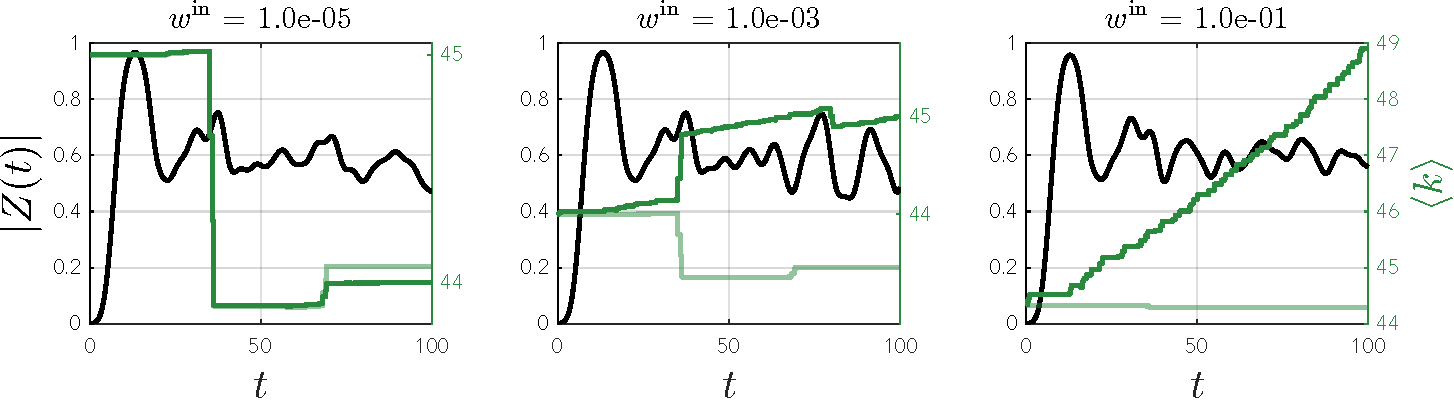
\includegraphics[width = \textwidth]{../Figures/Learning/KempterWinWout.pdf}
\caption{Tuning of the hyperparameters $w^{\mathrm{in}}$ and $w^{\mathrm{out}}$. Left: the learning dynamics with zero weights, as a benchmark. Middle: the learning dynamics for small, non-zero weights. The mean coupling strength is higher, but the overall synchronisation is lower. This might yield an interesting topological structure. Right: the learning dynamics with the same magnitude as the learning window disturb the learning process.}
\label{fig:KempterWinWout}
\end{figure}


\subsection{Results}
\begin{figure}[H]
\centering
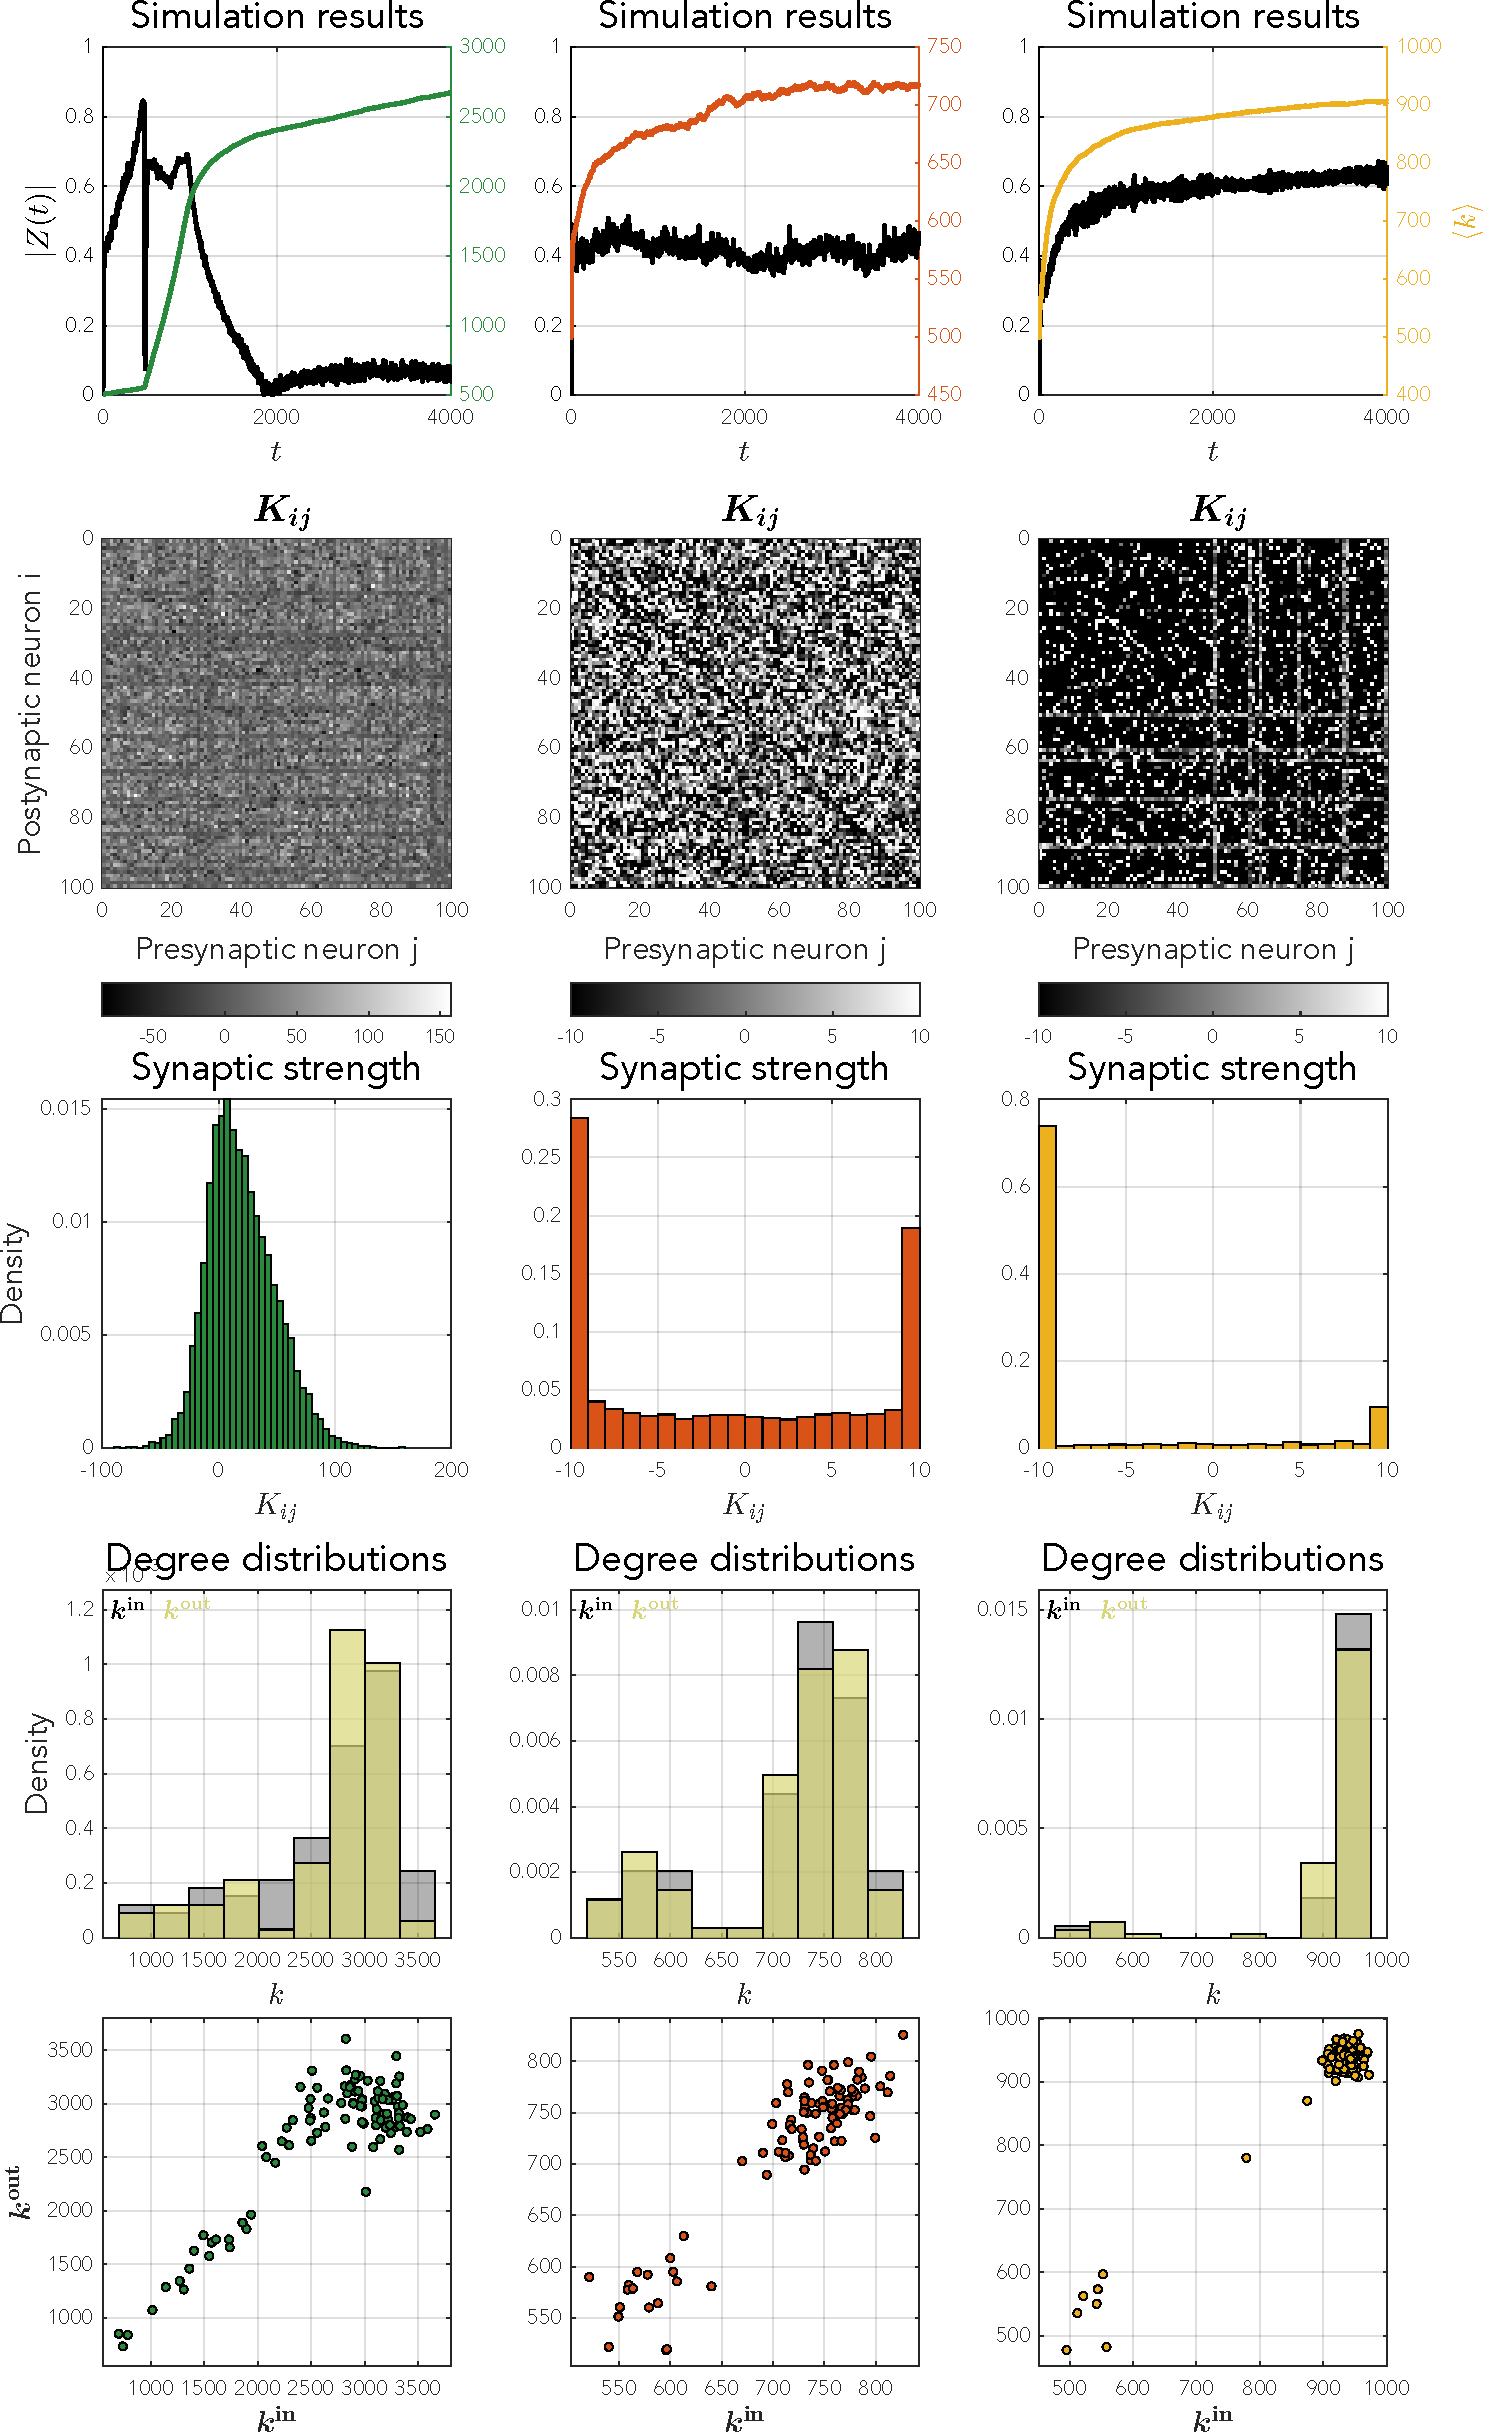
\includegraphics[height = \textheight]{../Figures/Learning/STDP.pdf}
\caption{Results of the \STDP learning.}
\label{fig:STDP}
\end{figure}

\begin{figure}[H]
\centering
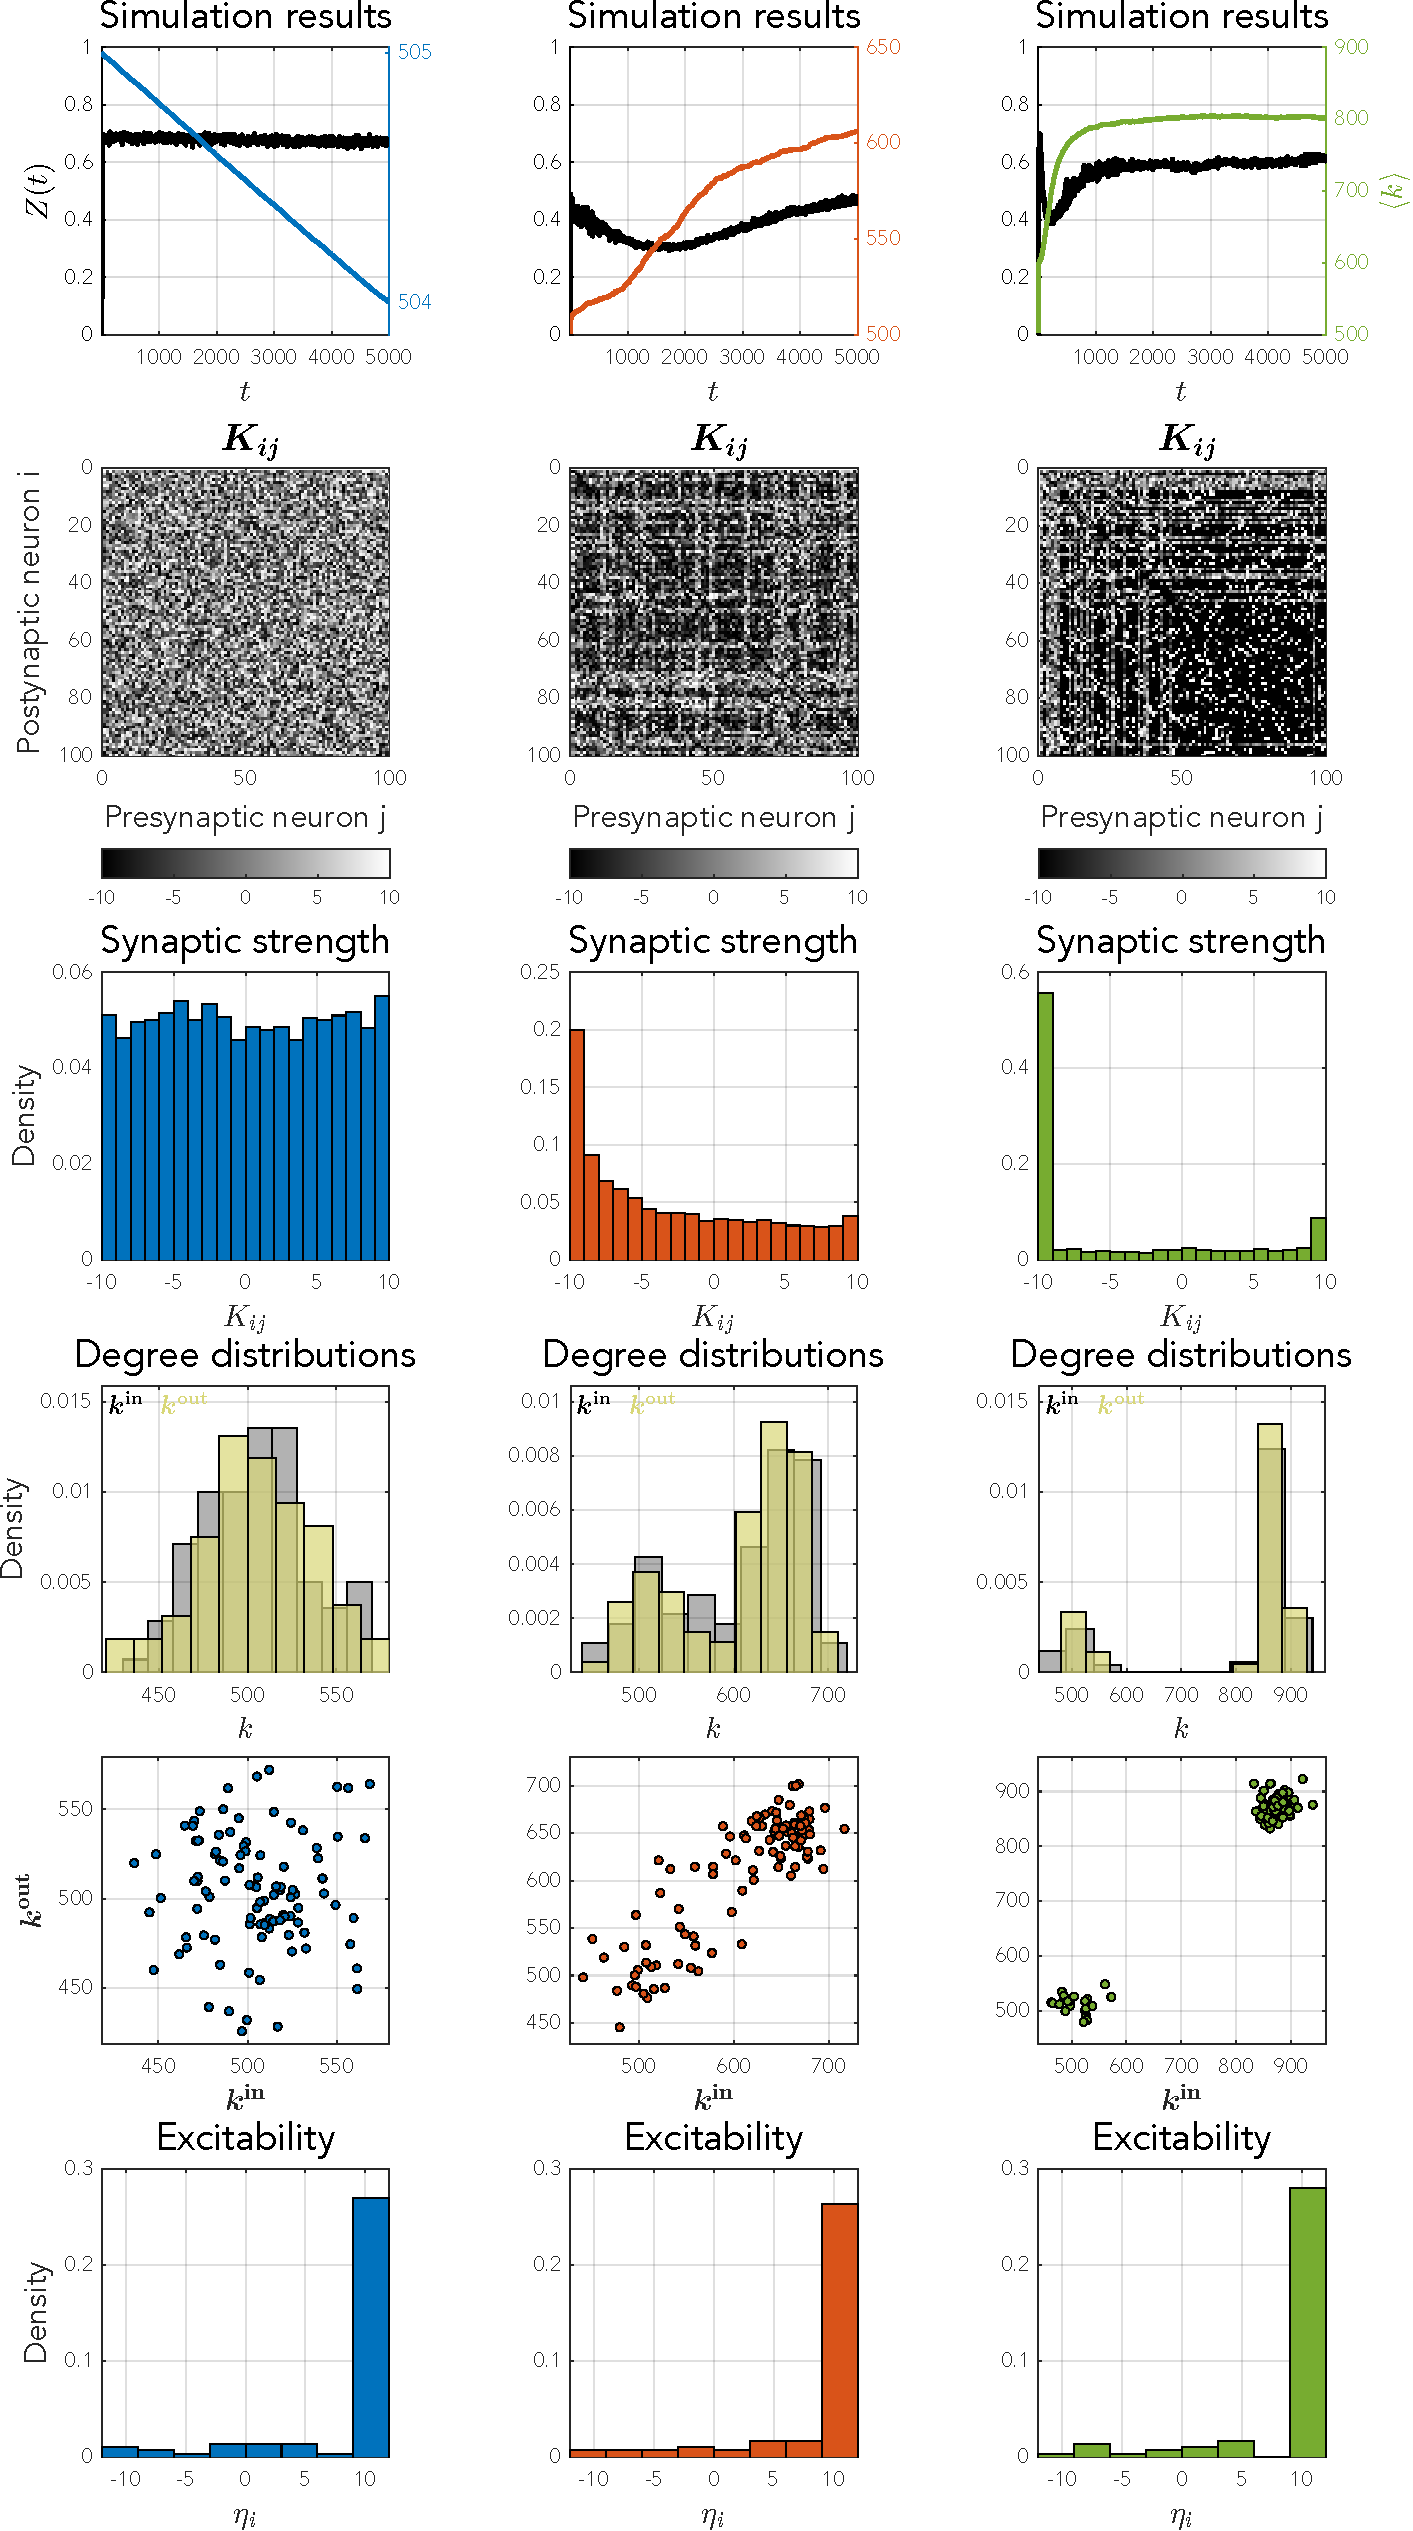
\includegraphics[height = \textheight]{../Figures/Learning/STDPandIP.pdf}
\caption{Results of the \STDP learning with \IP learning.}
\label{fig:STDP}
\end{figure}

\subsection{Results}
\textcolor{red}{TODO}: \textsl{describe the emergent behaviour.}

